\section{Polarization Cameras in the Maritime Domain}
Light behaves as a transverse wave, with its electromagnetic field oscillating in a plane perpendicular to the direction in which it travels.
With color filters the different frequencies of the ocsillation can be separated, and we can generate RGB images that make it easy to separate a red boat from a blue sea.
In a similar way, linear polarization filters can be used to separate light into its different polarization directions, which gives us a new set of tools to analyze the scene.


\subsection{Polarization Properties of Reflected Light}
When light is reflected off a surface, its polarization state changes \cite[34]{lingUniversityPhysicsVolume2016}.
This is illustrated in Figure \ref{fig:polarized_reflection} where the unpolarized light reflected off a surface becomes partially polarized.


\begin{figure}[H]
    \centering
    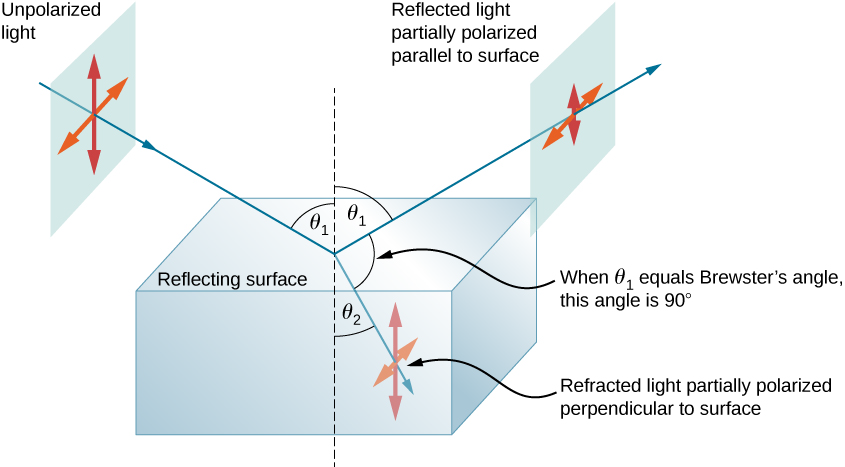
\includegraphics[width=.8\linewidth]{figures/polarization/reflaction.png}
    \caption{Polarization by reflection.
        \cite[Figure 1.38]{lingUniversityPhysicsVolume2016}}
    \label{fig:polarized_reflection}
\end{figure}


Unpolarized light can be described as a sum of two orthogonal linear polarizations $R_\perp$ and $R_\parallel$, where $R_\perp$ is perpendicular to the plane of incidence and $R_\parallel$ is parallel to the plane of incidence  \cite{FresnelEquations2024}.
These two components are referred to as s-polarized and p-polarized light, respectively.
Their reflection coefficients differ and are given by the Fresnel equations below \cite{FresnelEquations2024}:

\begin{align}
    R_\perp =         & \left|{\frac {n_{1}\cos \theta _1-n_{2}\cos \theta _2}{n_{1}\cos \theta _1+n_{2}\cos \theta _2}}\right|^{2}
                      &
    R_\parallel     = & \left|{\frac {n_{1}\cos \theta _2-n_{2}\cos \theta _1}{n_{1}\cos \theta _2+n_{2}\cos \theta _1}}\right|^{2}
\end{align}

Where  $\eta_1$ and $\eta_2$ are the refractive indices of the two media,
$\theta_i$ is the angle of incidence and $\theta_r$ is the angle of refraction.
Using the trigonometric identity $ \cos^2{\left(\theta_2 \right)} = 1- \sin^2{\left(\theta_2 \right)}$ and Snell's law $\eta_1 \sin{\left(\theta_1 \right)} = \eta_2 \sin{\left(\theta_2 \right)}$ the angle of refraction, $\theta_2$ can be removed, and the equations can be rewritten as:

\begin{align}
    R_\perp =         & \left|{\frac {n_{1}\cos \theta _1-n_{2}{\sqrt {1-\left({\frac {n_{1}}{n_{2}}}\sin \theta _1\right)^{2}}}}{n_{1}\cos \theta _1+n_{2}{\sqrt {1-\left({\frac {n_{1}}{n_{2}}}\sin \theta _1\right)^{2}}}}}\right|^{2}
                      &
    R_\parallel     = & \left|{\frac {n_{1}{\sqrt {1-\left({\frac {n_{1}}{n_{2}}}\sin \theta _1\right)^{2}}}-n_{2}\cos \theta _1}{n_{1}{\sqrt {1-\left({\frac {n_{1}}{n_{2}}}\sin \theta _1\right)^{2}}}+n_{2}\cos \theta _1}}\right|^{2}
\end{align}


Inserting the refractive index of air, $n_1 = 1$, and the refractive index of water, $n_2 = 1.33$, the reflectance can be calculated and plotted as a function of the angle of incidence, $\theta_1$, alone as shown in Figure \ref{fig:brewster0}.
The \gls{dolp} is the degree to which light is polarized and can be defined as the ratio between the difference and the sum of the two polarizations components.
The \gls{dolp} is plotted in Figure \ref{fig:brewster1}.
At one particular angle of incidence, $\theta_B$, known as the Brewser angle, $R_\parallel$ becomes zero, and the reflected light is completely s-polarized \cite{BrewsterAngle2024}:
\begin{align}
    \theta_B & = \arctan{\frac{n_2}{n_1}} & DoLP= & \frac{\left | R_\perp - R_\parallel \right |}{R_\perp + R_\parallel}
\end{align}

\begin{figure}[H]
    \centering
    \begin{subfigure}{.5\textwidth}
        \centering
        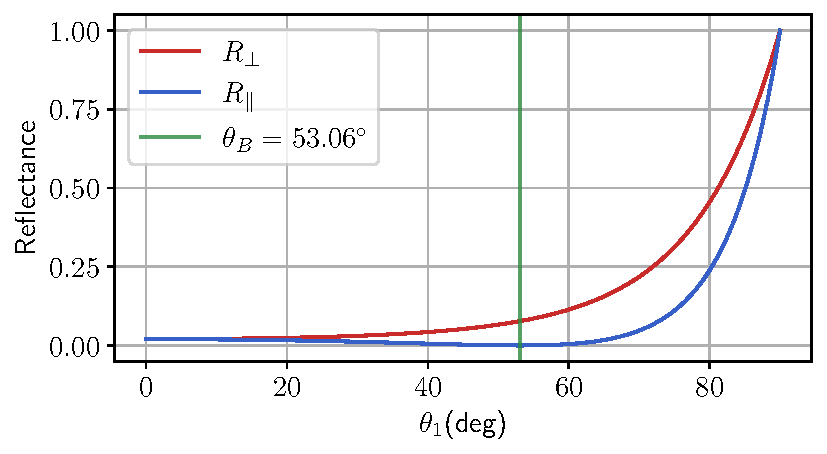
\includegraphics[width=\textwidth]{figures/pol_plots/brewster0.pdf}
        \caption{Reflectance of S and P polarized light of water.}
        \label{fig:brewster0}
    \end{subfigure}%
    \begin{subfigure}{.5\textwidth}
        \centering
        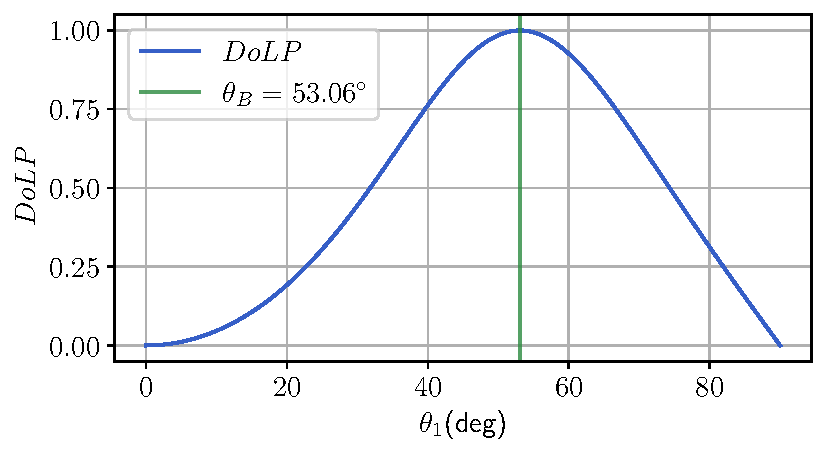
\includegraphics[width=\textwidth]{figures/pol_plots/brewster1.pdf}
        \caption{\gls{dolp} of light reflected off water.}
        \label{fig:brewster1}
    \end{subfigure}
    \caption{Reflectance and \gls{dolp} of light reflected off water as a funcion of of the angle of incidence.
        The Brewster angle is marked with a vertical line.}
    \label{fig:test}
\end{figure}




\subsection{Polarization of Light}
In the case of polarized light, the electromagnetic oscillations trace an elliptical path, which simplifies to a circular or straight line for pure circular or linear polarization, respectively.
When light passes through a linear polarizer, the electric field is filtered, allowing only the component aligned with the polarizer to continue through.
By aligning four linear polarizers at 45-degree intervals, the degree of linear polarization (\gls{dolp}) and the angle of linear polarization (\gls{aolp}) can be determined as shown in Figure \ref{fig:polarization_calculation}.

\begin{figure}[H]

    \begin{minipage}{.48\textwidth}
        % \begin{figure}[H]
        % \centering
        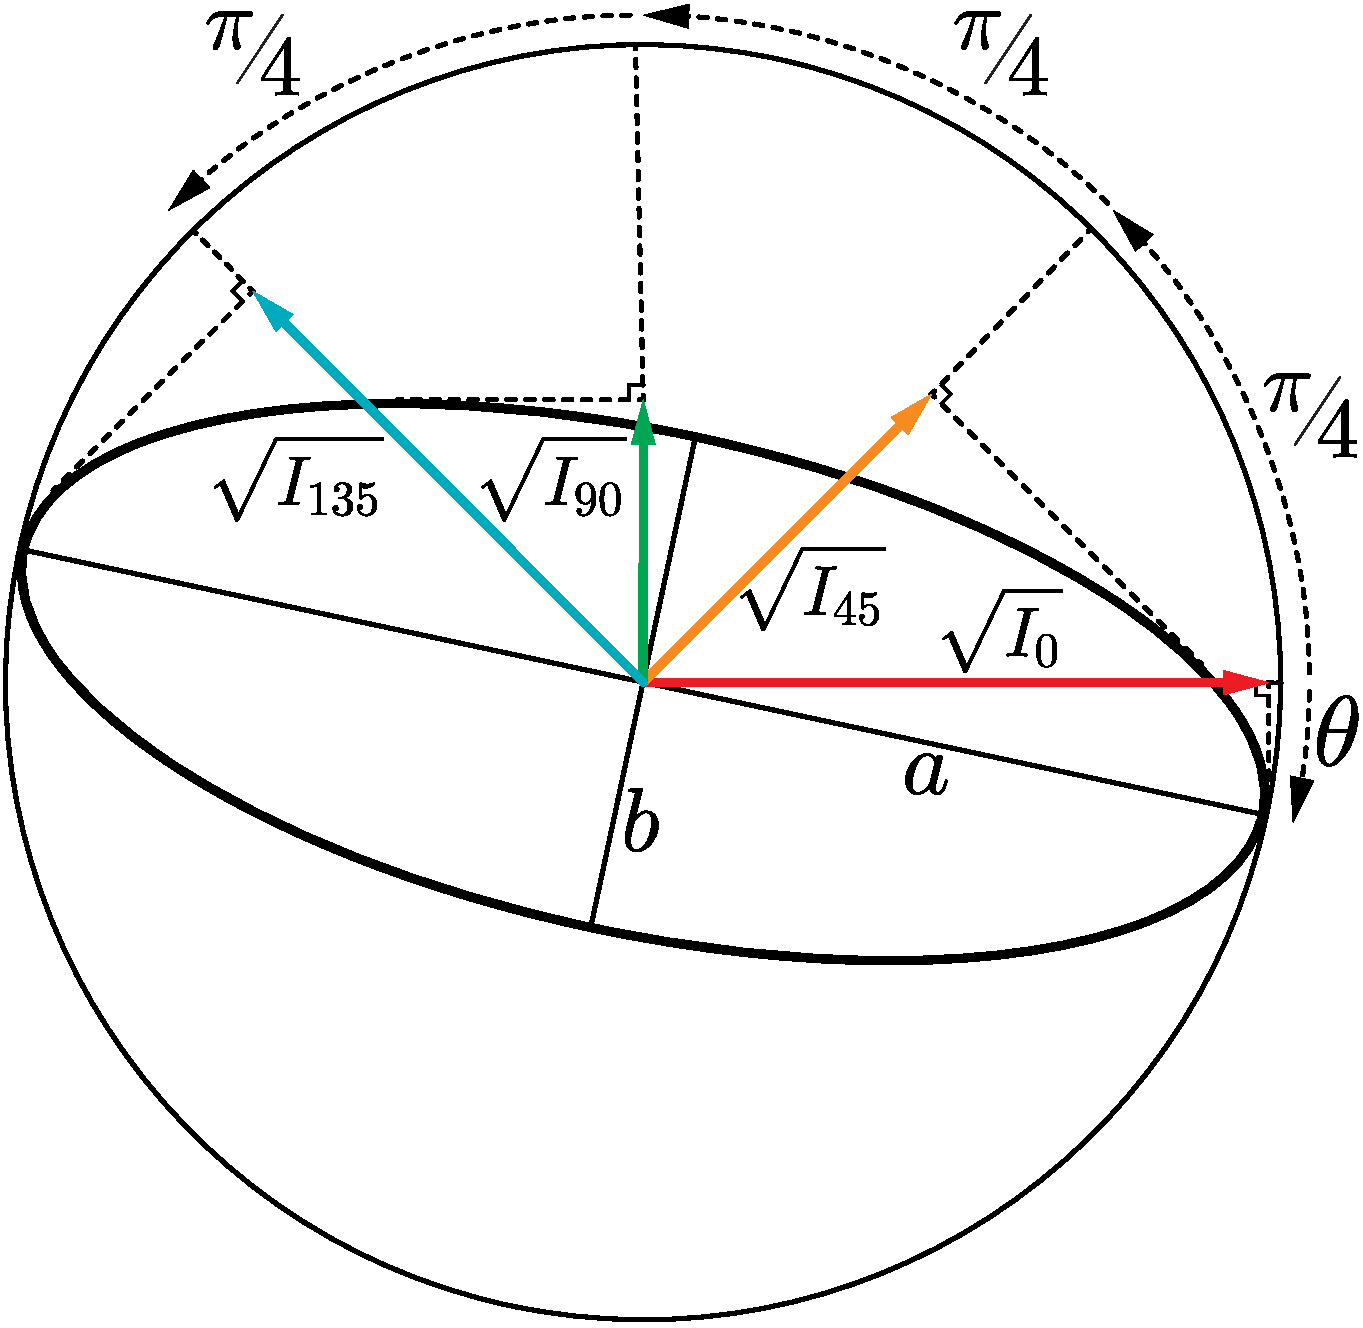
\includegraphics[width=\textwidth]{figures/polarization_sketch.pdf}
        % \label{fig:polarization_naming}
        % \end{figure} 
    \end{minipage}
    \hfill
    \begin{minipage}{.48\textwidth}
        \begin{alignat}{3}
             & \mathrlap{\cos\theta \cdot a\cos t -  \sin\theta \cdot b\sin t}                &
             &                                                                                &
             &                                                                                  \\
             &                                                                                &
             & = \mathrlap{\sqrt{a^2\cos^2\theta+b^2\sin^2\theta} \cos(\omega + \phi)}        &
             &                                                                                  \\[1em]
             & I_0                                                                            &
             & = \mathrlap{a^2\cos^2\theta + b^2\sin^2\theta                                } &
             &                                                                                  \\
             & I_{45}                                                                         &
             & = \mathrlap{a^2\cos^2(\theta-\frac{\pi}{4}) + b^2\sin^2(\theta-\frac{\pi}{4})} &
             &                                                                                  \\
             & I_{90}                                                                         &
             & = \mathrlap{a^2\sin^2\theta + b^2\cos^2\theta                                } &
             &                                                                                  \\
             & I_{135}                                                                        &
             & = \mathrlap{a^2\sin^2(\theta-\frac{\pi}{4}) + b^2\cos^2(\theta-\frac{\pi}{4})} &
             &                                                                                  \\[1em]
             & S_0                                                                            &
             & = I_0 + I_{90}                                                                 &
             & = a^2+b^2                                                                        \\
             & S_1                                                                            &
             & = I_0 - I_{90}                                                                 &
             & =(a^2-b^2)\cos(2x)                                                               \\
             & S_2                                                                            &
             & = I_{45} - I_{135}                                                             &
             & =(a^2-b^2)\sin(2x)                                                               \\[1em]
             & DoLP                                                                           &
             & =\frac{a^2-b^2}{a^2+b^2}                                                       &
             & = \frac{\sqrt{S_1^2 + S_2^2}}{S_0}                                               \\
             & AoLP                                                                           &
             & =  \theta                                                                      &
             & = \frac{1}{2}\arctan{\left(\frac{S_2}{S_1}\right)}
        \end{alignat}
    \end{minipage}%

    \caption{How four linear polarizers placed at $45^\circ$ intervals can be used to calculate the \gls{dolp} and \gls{aolp} of polarized light. The intensities  \label{fig:polarization_calculation}}
\end{figure}

\begin{figure}[H]
    \begin{subfigure}[T]{.48\textwidth}
        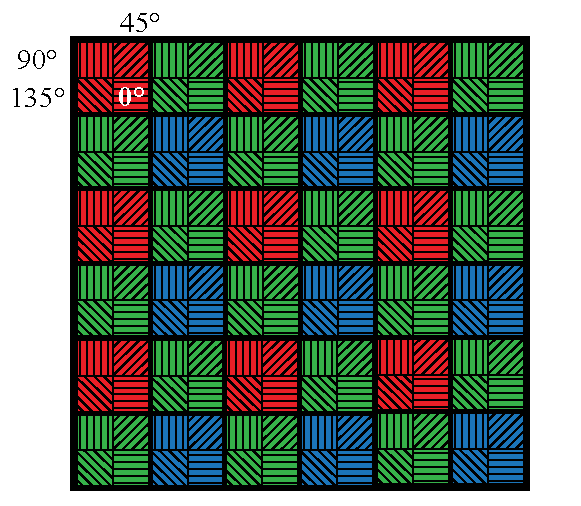
\includegraphics[width=\textwidth]{figures/sensor_layout.pdf}
        \caption{A 12\times12 slice of the color polarization filter array sensor. \label{fig:cpfa}}
    \end{subfigure}%
    \hfill
    \begin{subfigure}[T]{.48\textwidth}
        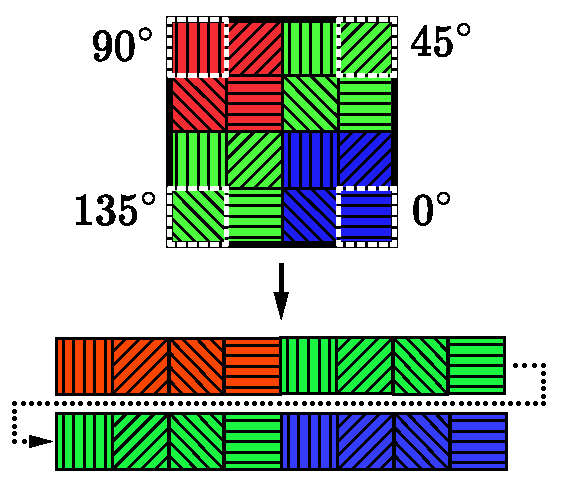
\includegraphics[width=\textwidth]{figures/sensor_packaging.pdf}
        \caption{The 12\times12 raw data from \ref{fig:cpfa}) can be reordered as a 3\times3 image with 16 channels.}
    \end{subfigure}
    \caption{Visualization of a color polarization filter array sensor with a RGGB Bayer pattern and a $90^\circ$ $45^\circ$ $135^\circ$ $0^\circ$ polarization filter subdivision.
        \label{fig:polarization_naming}}
\end{figure}

\begin{figure}[H]
    \centering
    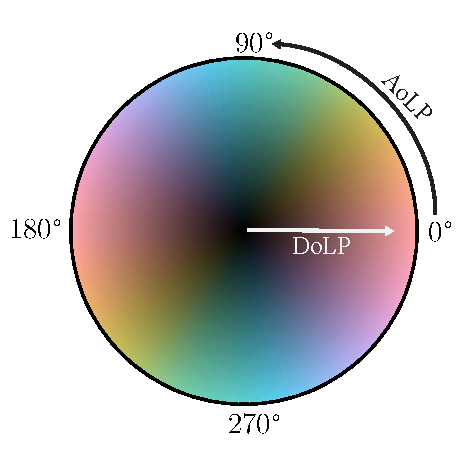
\includegraphics[width=0.4\textwidth]{figures/cmap/aolp_dolp_cmap.pdf}
    \caption{Visualization of \gls{dolp} and \gls{aolp}}
\end{figure}

\subsection*{Debayering}
There are other more advanced methods but a simple convolution works.



% \section{Debayering of Color Polarization Images}

% \begin{align*}
%     \text{BT709} = \begin{bmatrix}
%                        0.2126  & 0.7152  & 0.0722  \\
%                        -0.1146 & -0.3854 & 0.5     \\
%                        0.5     & -0.4542 & -0.0458
%                    \end{bmatrix}
% \end{align*}


